\chapter{Klasifiasi Teks}
\section{Jesron Marudut Hatuan/1164077}

\subsection{Teori}
\begin{enumerate}
\item Pengertian Klasifikasi teks
\par Klasifikasi merupakan sebuah kata serapan yang berasal dari bahasa Belanda, yaitu classificatie, yang sendirinya berasal dari bahasa Prancis classification. Istilah ini menunjuk pada metode untuk menyusun data secara sistematis atau menurut beberapa aturan atau kaidah yang telah ditetapkan.
Di dalam kamus besar bahasa Indonesia, klasifikasi adalah penyusunan bersistem dalam kelompok atau golongan menurut kaidah atau standar yang ditetapkan. Secara harafiah bisa pula dikatakan bahwa klasifikasi adalah pembagian sesuatu menurut kelas-kelas. Menurut Ilmu Pengetahuan, Klasifikasi adalah Proses pengelompokkan benda berdasarkan ciri-ciri dari persamaan dan perbedaan.
\begin{figure}[ht]
\centering
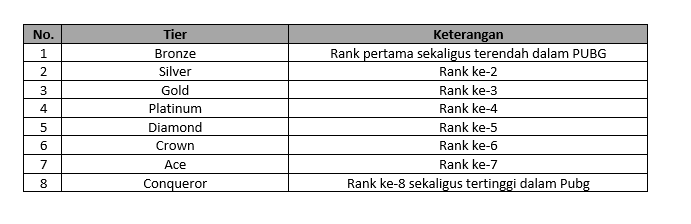
\includegraphics[scale=0.5]{figures/ch4/1.png}
\caption{Klasifikasi teks}
\label{Ilustrasi Klasifikasi Teks}
\end{figure}
	
\item Alasan Klasfikasii Bunga tidak bisa menggunakan machine learning
\par Machine Learning tidak dapat mengklasifikasikan bunga, dikarena data yang diberikan pada  mesin itu akan di algoritmakan untuk mencari sesuatu yang menarik dalam data yang kita berikan, hingga akhirnya sistem AI akan membangun pengetahuan berdasarkan data tersebut. Dengan maksud pembelajaran mesin data beradaptasi terhadap suatu masalah dengan mempelajari pola-pola yang ditemukan dalam data. Sebagai contoh data pada spesies bunga dari genus Iris dengan melihat ukuran sepal (kelopak) dan mahkota pada algoritma data bunga tersebut akan melatih proses pembelajaran pada mesin dalam menganalisa spesies bunga Iris. Dan algoritma pembelajaran mesin akan mempelajari karakteristik dari masing-masing spesies bunga Iris berdasarkan ukuran sepal dan petal yang diberikan.
\begin{figure}[ht]
\centering
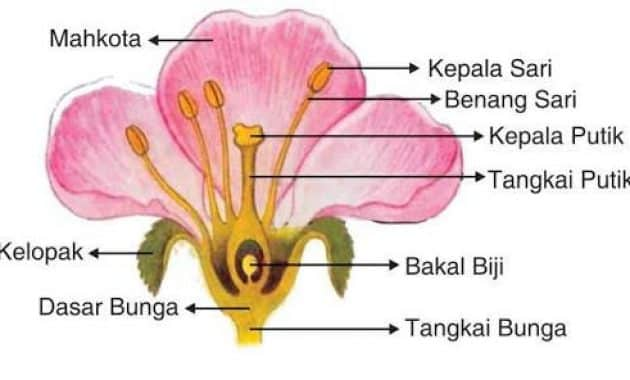
\includegraphics[scale=0.5]{figures/ch4/2.jpg}
\caption{Klasifikasi bunga}
\label{Ilustrasi Klasifikasi Bunga}
\end{figure}

\item
Youtube memungkinkan agar mendapatkan video yang direkomendasikan, karena Machine Learning pada Youtube pasti akan melibatkan data yang sering di lihat oleh penggunanya. Youtube juga akan memberitahukan si pengguna apabila ada video baru yang telah di upload pada chanel yang direkomendasikan untuk si pengguna. Dan apabila menonton video pada youtube maka youtube dapat mengingat dan menggunakan kata tersebut sebagai referensi.

\item Vectorisasi Data
\begin{itemize}
\item proses vektorisasi ini menghasilkan suatu wujud peta yang menggambarkan keadaan permukaan bumi atau bentang alam. Sifat data yang geometris menunjukkan ukuran dimensi yang sesungguhnya.
\end{itemize}
	
\item Bag of word
\par Bag of word merupakan konsep yang diambil dari analisis, kemudian merepresentasikan dokumen berupa kumpulan informasi penting tanpa mengurutkan setiap katanya.
\begin{figure}[ht]
\centering
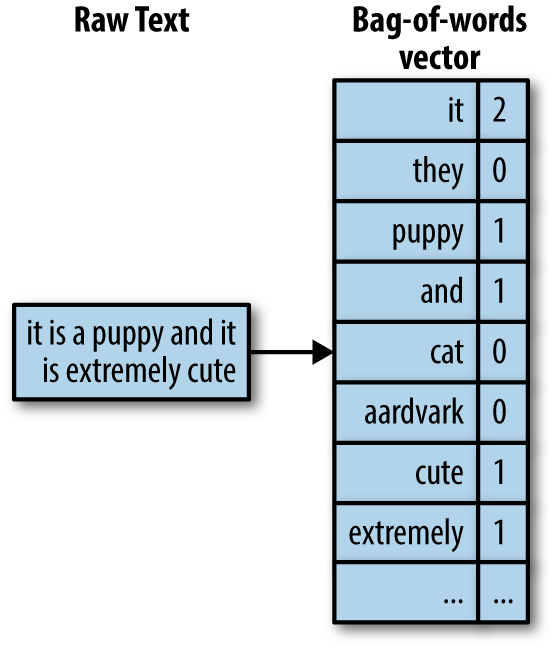
\includegraphics[scale=0.5]{figures/ch4/5.png}
\caption{Bag of Word}
\label{Contoh Ilustrasi}
\end{figure}
	
\item TF-IDF
\par TF-IDF dimaksudkan untuk mencerminkan seberapa relevan suatu istilah dalam dokumen yang diberikan. Intuisi di baliknya adalah bahwa jika sebuah kata muncul beberapa kali dalam sebuah dokumen, kita harus meningkatkan relevansinya karena itu harus lebih bermakna daripada kata-kata lain yang muncul lebih sedikit kali (TF). Pada saat yang sama, jika sebuah kata muncul berkali-kali dalam suatu dokumen tetapi juga di sepanjang banyak dokumen lain, mungkin itu karena kata ini hanya kata yang sering; bukan karena itu relevan atau bermakna (IDF).
\begin{figure}[ht]
\centering
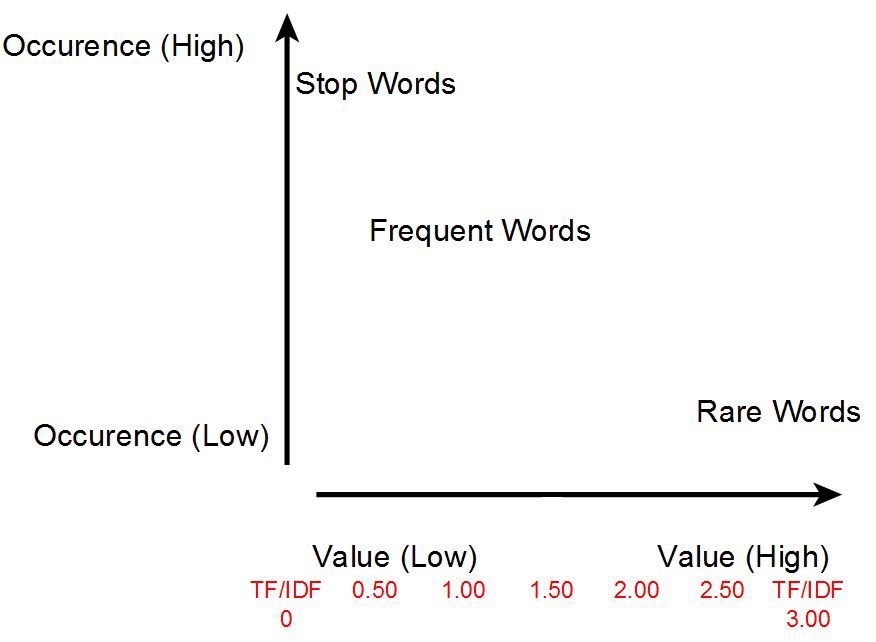
\includegraphics[scale=0.5]{figures/ch4/6.jpeg}
\caption{TF-IDF}
\label{Contoh Ilustrasi}
\end{figure}
\end{enumerate}


\section{Jesron Marudut Hatuan / 1164077}

\subsection{Praktek}
\begin{enumerate}
\item Kali ini saya akan membuat data dummy dimana saya menggunakannya dengan format csv, dan data-datanya saya ambil dari sebuah web yang bernama UCI Machine Learning
\par Repository dengan nama file Youtube03-LMFAO.csv
\begin{figure}[ht]
\centerline{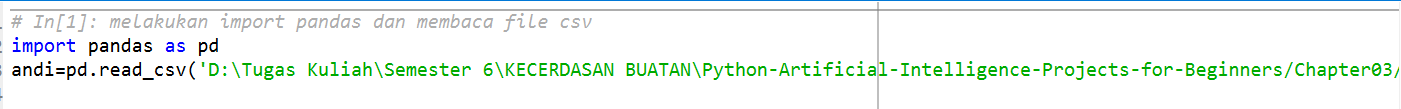
\includegraphics[width=1\textwidth]{figures/c4P/1.PNG}}
\caption{Data Dummy 500 Data}
\label{Contoh Ilustrasi}
\end{figure}

\subitem Penjelasan pada gambar 1 yaitu mengimport library pandas dimana kita mengaliaskan praktek sebagai pandas. Pandas berguna untuk mengelola  dataframe = matrix = tabel kemudian untuk memanggil nama alias dan membaca format csvnya.
\item Dari dataframe yang sudah ada sebelumnya kita akan membagi menjadi 2 yaitu 450 row pertama dan 50 row 
\par Dapat dilihat pada gambar \ref{2}
\begin{figure}[ht]
\centerline{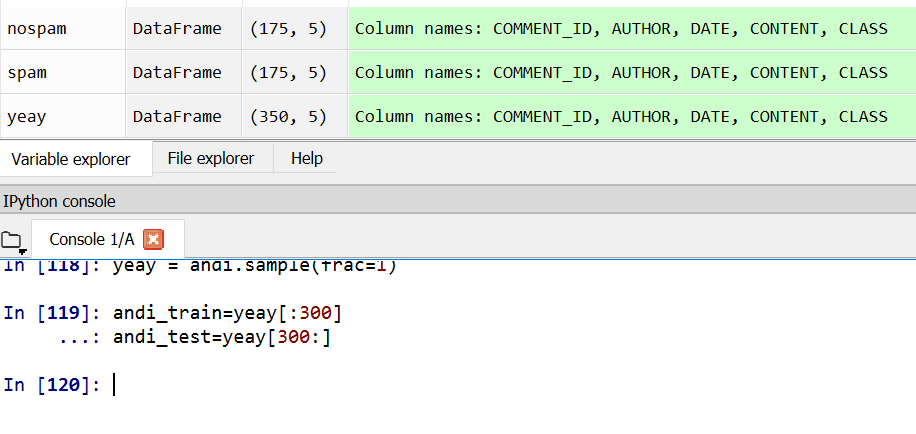
\includegraphics[width=1\textwidth]{figures/c4P/2.PNG}}
\caption{Membagi 2 Dataframe}
\label{Contoh Ilustrasi}
\end{figure}

\subitem Penjelasan pada gambar 2 yaitu baris pertama dimana d\_train untuk membagi data training sebanyak 450 row dan pada 
\par baris kedua dimana d\_test untuk data sisa atau data yang baru sebanyak 50 row.
\item Melakukan Vektorisasi dan Klasifikasi Data pada data LMFAO pada gambar 3  merupakan dataframe keseluruhan dari file csv yang sudah dimasukkan dengan jumlah 448 baris dan 5 kolom. Nospam merupakan dataframe yang isinya hanya data yang bukan termasuk spam dengan inisial angka 0. Sedangkan spam merupakan dataframe yang isinya hanya data spam dengan inisial angka 1.
\begin{figure}[ht]
\centerline{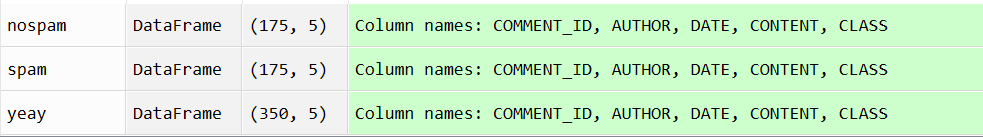
\includegraphics[width=1\textwidth]{figures/c4P/3.PNG}}
\caption{Vektorisasi dan Klasifikasi Data}
\label{Contoh Ilustrasi}
\end{figure}

\subitem  Pada gambar 3 merupakan hasil output content dimana terdapat 448 baris/data yang mempunyai 1602 kata-kata yang digunakan pada komentar yang ada di content tersebut.
\begin{figure}[ht]
	\centerline{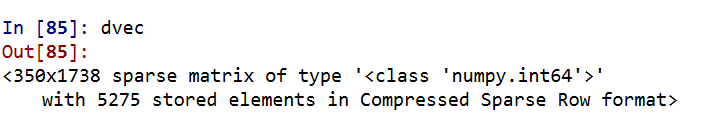
\includegraphics[width=1\textwidth]{figures/c4P/4.PNG}}
	\caption{Data Content}
	\label{Contoh Ilustrasi}
\end{figure}

\subitem Pada gambar 4 maksud dari outputannya merupakan dataframe kata-kata tadi yang berjumlah 1602 kata orang 
 yang komen pada data LMFAO.
\begin{figure}[ht]
	\centerline{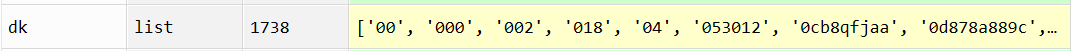
\includegraphics[width=1\textwidth]{figures/c4P/5.PNG}}
	\caption{DataFrame Kata-kata Pada Content}
	\label{Contoh Ilustrasi}
\end{figure}

\item Mengklasifikasikan dari data vektorisasi dengan menggunakan klasifikasi svm(support vektorisasi machine) dapat dilihat pada  gambar 6.
\begin{figure}[ht]
	\centerline{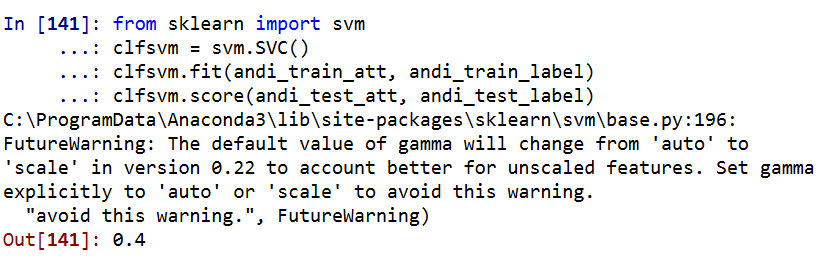
\includegraphics[width=1\textwidth]{figures/c4P/6.PNG}}
	\caption{Klasifikasi SVM Dari Data Vektorisasi}
	\label{Contoh Ilustrasi}
\end{figure}

\subitem Jadi pada gambar 6 merupakan hasil dari memprediksi data score vektorisasi dengan svm menggunakan metode fit dimana digunakan untuk data training atau data pelatihannya.
\item Mengklasifikasikan dari data vektorisasi dengan menggunakan klasifikasi Decision Tree dapat dilihat pada gambar 7.
\begin{figure}[ht]
	\centerline{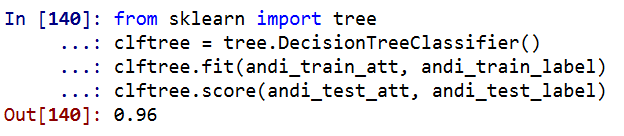
\includegraphics[width=1\textwidth]{figures/c4P/7.PNG}}
	\caption{Klasifikasi Decision Tree Dari Data Vektorisasi}
	\label{Contoh Ilustrasi}
\end{figure}

\subitem Jadi pada gambar 7 merupakan hasil dari memprediksi data score vektorisasi dengan Decision Tree menggunakan metode fit dimana digunakan untuk data training atau data pelatihannya saja.
\item Mengeplot confusion matrix menggunakan matplotlib dapat dilihat pada gambar 8.
\begin{figure}[ht]
	\centerline{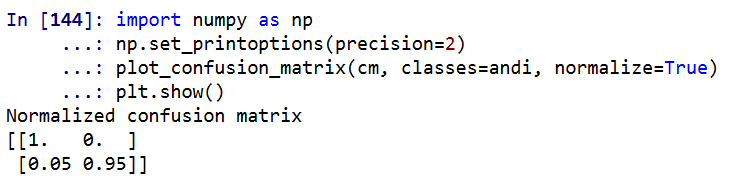
\includegraphics[width=1\textwidth]{figures/c4P/8.PNG}}
	\caption{Plot Confusion Matrix Menggunakan Matplotlib}
	\label{Contoh Ilustrasi}
\end{figure}

\subitem Pada gambar 8 sebelumnya kita harus mengimport matplotlibnya terlebih dahulu setelah itu di sini saya 
 menggunakan numpy untuk mengeluarkan hasil plot confusion matrix pada matplolibnya nantinya akan keluar normalisasi dari  confusion matrix berupa data baris dan kolom. 
\item Menjalankan program cross validation pada data vektorisasi dapat dilihat pada gambar 9.
\begin{figure}[ht]
	\centerline{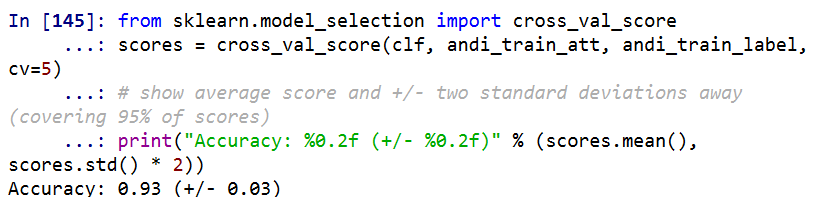
\includegraphics[width=1\textwidth]{figures/c4P/9.PNG}}
	\caption{Program Cross Validation Pada Data Vektorisasi}
	\label{Contoh Ilustrasi}
\end{figure}

\subitem Pada gambar 9 yang pertama yaitu memunculkan akurasi cross validation dari random forest pada data yang sudah divektorisasi, yang kedua yaitu memunculkan akurasi cross validation dari decision tree pada data yang sudah divektorisasi, dan yang ketiga yaitu memunculkan akurasi cross validation dari svm pada data yang sudah divektorisasi.
\item Membuat program pengamatan komponen informasi pada data yang sudah divektorisasi dapat dilihat pada gambar 10
\begin{figure}[ht]
	\centerline{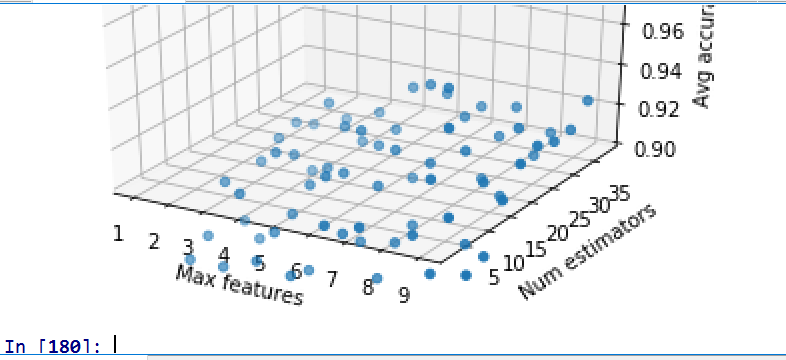
\includegraphics[width=1\textwidth]{figures/c4P/10.PNG}}
	\caption{Program Pengamatan Komponen Informasi}
	\label{Contoh Ilustrasi}
\end{figure}

\subitem Pada gambar 10  merupakan hasil outputan yang mana max features di sana terdapat 9 data dari 10 yang sudah kita masukkan ke dalam codingan sebelumnya dan penomoran estimatornya merupakan data per 5 dari angka 40 sedangkan rata-rata akurasinya kita tuliskan datanya mulai dari 0.9 sampai dengan 1. Titik-titik yang didalam tersebut merupakan data vektorisasi dari pengamatan komponen informasinya.
\end{enumerate}

\subsection{Penanganan Eror}
\begin{enumerate}
\item Pada gambar 11 merupakan ScreeShootan dari data yang eror.
\begin{figure}[ht]
	\centerline{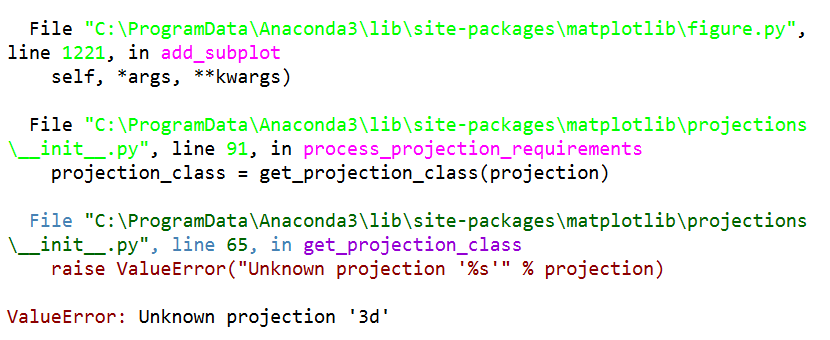
\includegraphics[width=1\textwidth]{figures/c4P/11.PNG}}
	\caption{Eror matplotlib.pyplot}
	\label{c4_16}
\end{figure}

\item 
\begin{verbatim}
 matplotlib.pyplot
Traceback (most recent call last):

  File "<ipython-input-151-8094433808cc>", line 6, in <module>
    ax = fig.gca(projection='3d')

  File "C:\ProgramData\Anaconda3\lib\site-packages\matplotlib\figure.py", line 1817, in gca
    return self.add_subplot(1, 1, 1, **kwargs)

  File "C:\ProgramData\Anaconda3\lib\site-packages\matplotlib\figure.py", line 1221, in add_subplot
    self, *args, **kwargs)

  File "C:\ProgramData\Anaconda3\lib\site-packages\matplotlib\projections\_init_.py", line 91, in process_projection_requirements
    projection_class = get_projection_class(projection)

  File "C:\ProgramData\Anaconda3\lib\site-packages\matplotlib\projections\_init_.py", line 65, in get_projection_class
    raise ValueError("Unknown projection '%s'" % projection)

ValueError: Unknown projection '3d'

<Figure size 432x288 with 0 Axes>
\end{verbatim}

\item Solusi eror tersebut dengan menambahkan  menambahkan codingan tersebut seperti berikut.
\begin{verbatim}
from mpl_toolkits.mplot3d import Axes3D
from matplotlib import cm
fig = plt.figure()
fig.clf()
\end{verbatim}
\end{enumerate}